\documentclass[10 pt,usenames,dvipsnames, oneside]{article}
\usepackage{../../../modelo-ensino-medio}


\begin{document}

\begin{center}
  \begin{minipage}[l]{3cm}

\includegraphics[width=2cm]{logo}    
\end{minipage}\hfill
\begin{minipage}[r]{.8\textwidth}
 {\Large \scshape Atividade: Qual é o gráfico?}  
\end{minipage}
\end{center}
\vspace{.2cm}

\ifdefined\prof
\begin{objetivos}
\item \textbf{LAF1} Compreender função como uma relação de dependência entre duas variáveis, as ideias de domínio, contradomínio e imagem, e suas representações algébricas e gráficas e utilizá-las para analisar, interpretar e resolver problemas em contextos diversos, inclusive fenômenos naturais, sociais e de outras áreas.
\end{objetivos}

\begin{goals}
\begin{enumerate}

\item[OE1] Reconhecer comportamentos crescente e decrescente em funções a partir de sua representação gráfica.


\item[OE2] O “Para refletir”{} apresentado adiante, explora diferentes tipos de gráficos de funções decrescente e crescente. Procure fazer conexão desta atividade com esse “para Refletir”

\end{enumerate}
\tcblower

\begin{itemize}
\item Fazer a conexão com o “Para refletir”{} apresentado mais adiante, onde são explorados diferentes tipos de gráficos de função decrescente e crescente.

\item Como os gráficos são apenas esboços, mais importante que os valores da tabela são as suas variações.
\end{itemize}

\end{goals}

\bigskip
\begin{center}
{\large \scshape Atividade}
\end{center}
\fi

Dentre os gráficos apresentados a seguir identifique aquele que melhor descreve os dados apresentados em cada uma das tabelas seguintes.


\(a)\) Café esfriando
\begin{table}[H]
\centering
\begin{tabu} to \textwidth{|c|c|c|c|c|c|c|c|}
\hline
\cellcolor{primario}\textcolor{white}{\textbf{Tempo (minutos)}} & 0 & 5 & 10 & 15 & 20 & 25 & 30 \\
\hline
\cellcolor{primario}\textcolor{white}{\textbf{Temperatura ($^{\circ}$C)}} & 90 & 79 & 70 & 62 & 55 & 49 & 44\\
\hline
\end{tabu}
\end{table}

\(b)\) Preparando a ceia

\begin{table}[H]
\centering
\begin{tabu} to \textwidth{|c|c|c|c|c|c|c|c|}
\hline
\cellcolor{primario}\textcolor{white}{\textbf{Peso (quilos)}} & 3 & 4 & 5 & 6 & 7 & 8 & 9 \\
\hline
\cellcolor{primario}\textcolor{white}{\textbf{Tempo (horas)}} & 2,5 & 3 & 3,5 & 4 & 4,5 & 5 & 5,5\\
\hline
\end{tabu}
\end{table}

\(c)\) Depois de três canecas de cerveja…

\begin{table}[H]
\centering
\begin{tabu} to \textwidth{|c|c|c|c|c|c|c|c|}
\hline
\cellcolor{primario}\textcolor{white}{\textbf{Tempo (horas)}} & 1 & 2 & 3 & 4 & 5 & 6 & 7 \\
\hline
\cellcolor{primario}\textcolor{white}{\textbf{Álcool no sangue (mg/100ml)}} & 90 & 75 & 60 & 45 & 30 & 15 & 0 \\
\hline
\end{tabu}
\end{table}

\(d)\) Como um bebê cresce antes do nascimento

\begin{table}[H]
\centering
\begin{tabu} to \textwidth{|c|c|c|c|c|c|c|c|c|}
\hline
\cellcolor{primario}\textcolor{white}{\textbf{Tempo de gestação (meses)}} & 2 & 3 & 4 & 5 & 6 & 7 & 8 & 9 \\
\hline
\cellcolor{primario}\textcolor{white}{\textbf{Comprimento do bebê (cm)}} & 4 & 9 & 16 & 24 & 30 & 34 & 38 & 42 \\
\hline
\end{tabu}
\end{table}


\begin{figure}[H]
\centering

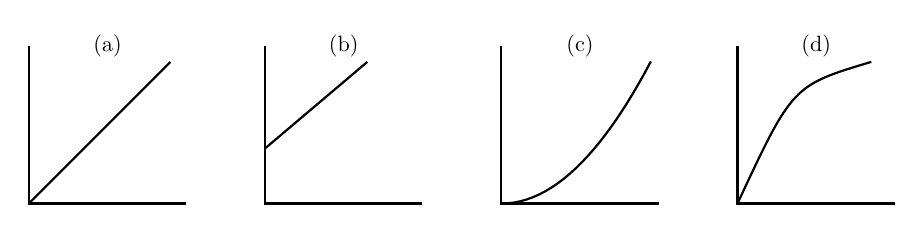
\begin{tikzpicture}
\draw[thick](0,2)--(0,0)--(2,0);
\draw(1,2)node[scale=.8]{(a)};
\draw[thick](0,0)--(1.8,1.8);
\begin{scope}[xshift=3cm]
\draw[thick](0,2)--(0,0)--(2,0);
\draw(1,2)node[scale=.8]{(b)};
\draw[thick](0,.7)--(1.3,1.8);
\begin{scope}[xshift=3cm]
\draw[thick](0,2)--(0,0)--(2,0);
\draw(1,2)node[scale=.8]{(c)};
\draw[domain=0:1.9,thick]plot(\x,.5*\x^2);
\begin{scope}[xshift=3cm]
\draw[thick](0,2)--(0,0)--(2,0);
\draw(1,2)node[scale=.8]{(d)};
\draw[thick](0,0).. controls (.7,1.5)..(1.7,1.8);
\end{scope}
\end{scope}
\end{scope}
\end{tikzpicture}

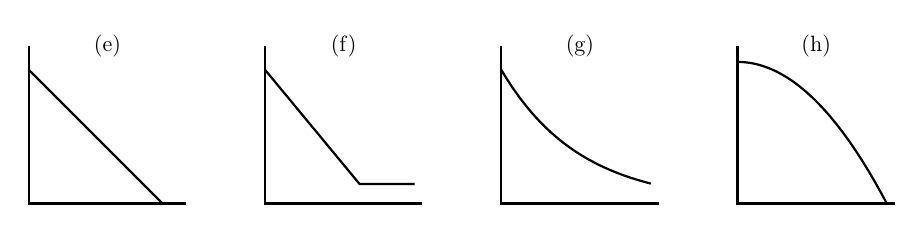
\begin{tikzpicture}
\draw[thick](0,2)--(0,0)--(2,0);
\draw(1,2)node[scale=.8]{(e)};
\draw[thick](0,1.7)--(1.7,0);
\begin{scope}[xshift=3cm]
\draw[thick](0,2)--(0,0)--(2,0);
\draw(1,2)node[scale=.8]{(f)};
\draw[thick](0,1.7)--(1.2,0.25)--(1.9,.25);
\begin{scope}[xshift=3cm]
\draw[thick](0,2)--(0,0)--(2,0);
\draw(1,2)node[scale=.8]{(g)};
\draw[domain=0:1.9,thick]plot(\x,{1.7*exp(-\x)});
\begin{scope}[xshift=3cm]
\draw[thick](0,2)--(0,0)--(2,0);
\draw(1,2)node[scale=.8]{(h)};
\draw[domain=0:1.9, thick]plot(\x,{(1.8-.5*\x^2} );
\end{scope}
\end{scope}
\end{scope}
\end{tikzpicture}

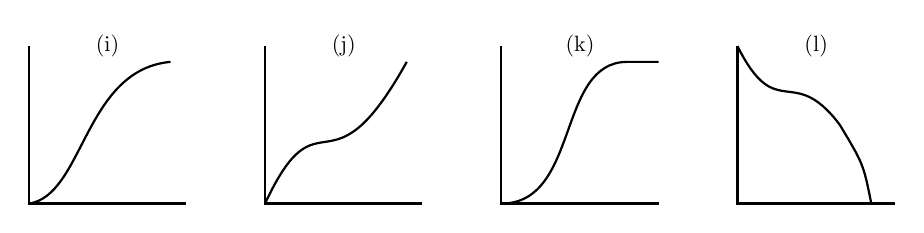
\begin{tikzpicture}
\draw[thick](0,2)--(0,0)--(2,0);
\draw(1,2)node[scale=.8]{(i)};
\draw[thick](0,0)..controls(.7,.1) and (.7,1.7) ..(1.8,1.8);
\begin{scope}[xshift=3cm]
\draw[thick](0,2)--(0,0)--(2,0);
\draw(1,2)node[scale=.8]{(j)};
\draw[thick](0,0)..controls(.7,1.5) and (.8,.0) ..(1.8,1.8);
\begin{scope}[xshift=3cm]
\draw[thick](0,2)--(0,0)--(2,0);
\draw(1,2)node[scale=.8]{(k)};
\draw[thick](0,0)..controls(1,0) and (.7,1.8) ..(1.6,1.8)..controls(1.9,1.8)..(2,1.8);
\begin{scope}[xshift=3cm]
\draw[thick](0,2)--(0,0)--(2,0);
\draw(1,2)node[scale=.8]{(l)};
\draw[thick](0,2)..controls(.5,1) and (.7,1.8) ..(1.3,1)..controls(1.6,.5)..(1.7,0);
\end{scope}
\end{scope}
\end{scope}
\end{tikzpicture}
\end{figure}

\(*\) Adaptado de \emph{The Language of Functions and Graphs}, Shell Centre for Mathematical Education Publications Ltd., 1985.

\ifdefined\prof
\begin{solucao}
\begin{enumerate}
\item (g)

\item (a)

\item (e) 

\item (k)

\end{enumerate}
\end{solucao}
\fi

\end{document}